% ******************************************************** %
%              TEMPLATE DE INFORME ORGA2 v0.1              %
% ******************************************************** %
% ******************************************************** %
%                                                          %
% ALGUNOS PAQUETES REQUERIDOS (EN UBUNTU):                 %
% ========================================
%                                                          %
% texlive-latex-base                                       %
% texlive-latex-recommended                                %
% texlive-fonts-recommended                                %
% texlive-latex-extra?                                     %
% texlive-lang-spanish (en ubuntu 13.10)                   %
% ******************************************************** %


\documentclass[a4paper]{article}
\usepackage[utf8]{inputenc}
\usepackage{charter}   % tipografia
\usepackage{graphicx}
%\usepackage{makeidx}
\usepackage{paralist} %itemize inline

\usepackage{float}
\usepackage{mathtools}
%\usepackage{amsmath, amsthm, amssymb}
%\usepackage{amsfonts}
%\usepackage{sectsty}
%\usepackage{charter}
\usepackage{wrapfig}
\usepackage{listings} % https://www.overleaf.com/learn/latex/Code_listing
\usepackage{bytefield}
\usepackage[english,spanish]{babel}
% \setcounter{secnumdepth}{2}
\usepackage{underscore}
\usepackage{caratula}
\usepackage{url}
\usepackage{hyperref}
\usepackage{graphicx}
\usepackage{amsmath}
\usepackage{algorithm}
\usepackage{algpseudocode}
\usepackage{titlesec}
\usepackage{tikz}
\usepackage{subcaption}
\usepackage{csquotes} % https://www.overleaf.com/learn/latex/typesetting_quotations

\usetikzlibrary{patterns,arrows,decorations.pathmorphing,backgrounds,positioning,fit,petri,decorations.pathreplacing}

\usetikzlibrary{arrows}

\DeclarePairedDelimiterX{\norm}[1]{\lVert}{\rVert}{#1}

% https://tex.stackexchange.com/questions/60209/how-to-add-an-extra-level-of-sections-with-headings-below-subsubsection
\setcounter{secnumdepth}{4}
\titleformat{\paragraph}
{\normalfont\normalsize\bfseries}{\theparagraph}{1em}{}
\titlespacing*{\paragraph}
{0pt}{3.25ex plus 1ex minus .2ex}{1.5ex plus .2ex}



\makeatletter
\def\BState{\State\hskip-\ALG@thistlm}
\makeatother

% ********************************************************* %
% ~~~~~~~~              Code snippets             ~~~~~~~~~ %
% ********************************************************* %

\usepackage{color} % para snipets de codigo coloreados
\usepackage{fancybox}  % para el sbox de los snipets de codigo


% ********************************************************* %
% ~~~~~~~~         Formato de las páginas         ~~~~~~~~~ %
% ********************************************************* %

\usepackage{fancyhdr}
\pagestyle{fancy}

%\renewcommand{\chaptermark}[1]{\markboth{#1}{}}
\renewcommand{\sectionmark}[1]{\markright{\thesection\ - #1}}

\fancyhf{}

\fancyhead[LO]{Sección \rightmark} % \thesection\ 
\fancyfoot[RO]{\thepage}
\renewcommand{\headrulewidth}{0.5pt}
\renewcommand{\footrulewidth}{0.5pt}
\setlength{\hoffset}{-0.8in}
\setlength{\textwidth}{16cm}
%\setlength{\hoffset}{-1.1cm}
%\setlength{\textwidth}{16cm}
\setlength{\headsep}{0.5cm}
\setlength{\textheight}{25cm}
\setlength{\voffset}{-0.7in}
\setlength{\headwidth}{\textwidth}
\setlength{\headheight}{13.1pt}

\renewcommand{\baselinestretch}{1.1}  % line spacing

% ******************************************************** %

% code style
\definecolor{codegreen}{rgb}{0,0.6,0}
\definecolor{codegray}{rgb}{0.5,0.5,0.5}
\definecolor{codepurple}{rgb}{0.58,0,0.82}
\definecolor{backcolour}{rgb}{0.95,0.95,0.92}

\lstdefinestyle{mystyle}{
    backgroundcolor=\color{backcolour},   
    commentstyle=\color{codegreen},
    %keywordstyle=\color{magenta},
    numberstyle=\tiny\color{codegray},
    stringstyle=\color{codepurple},
    %basicstyle=\ttfamily,
    breakatwhitespace=false,           
    breaklines=true,                 
    captionpos=b,                    
    % keepspaces=true,                 
    numbers=left,                    
    numbersep=5pt,                  
    % showspaces=false,                
    % showstringspaces=false,
    % showtabs=false,                  
    tabsize=4
}

\lstset{style=mystyle}

\begin{document}


\thispagestyle{empty}
\materia{Sistemas Operativos}
\submateria{Primer Cuatrimestre de 2020}
\titulo{Trabajo Práctico 1}
\subtitulo{\textit{Multithreading}}
\integrante{Manuel Panichelli}{72/18}{panicmanu@gmail.com}
\integrante{Vladimir Pomsztein}{364/18}{blastervla@gmail.com}
\integrante{Gaston Einan Rosinov}{37/18}{grosinov@gmail.com}

\maketitle
\newpage

\thispagestyle{empty}
\vspace{3cm}
\setcounter{tocdepth}{4}
\setcounter{secnumdepth}{5}
\tableofcontents

\section{Abstract}

Se aborda la problemática de programación de forma concurrente con \textit{POSIX threads}, en particular para una implementación de un \textit{HashMap} que cuenta la cantidad de apariciones de palabras en un conjunto de archivos. Además, se realiza un análisis del impacto en performance que trae aumentar el nivel de concurrencia.

\textit{\textbf{keywords:} POSIX, threads, concurrency, HashMap, List, synchronization, atomic, performance}

\section{Introducción}

Con la creciente exigencia técnica requerida para mejorar los procesadores modernos, de componentes cada vez más minúsculos, y el cada vez mayor uso de sistemas multiprogramables, el multiprocesamiento resulta una rama de estudio muy importante para la computación moderna. De ella se desprende el concepto de concurrencia, central en este estudio.

La concurrencia es una herramienta muy útil, ya que nos permite realizar tareas de forma más eficiente y veloz al poder distribuir la carga de procesamiento entre varios procesos o threads de un mismo programa; posibilita la paralelización de tareas, resultando en un potencial mejor rendimiento del programa o sistema. Sin embargo, estas ventajas no vienen sin sus propios problemas y dificultades, como lo son la contención entre los recursos, condiciones de carrera e inconsistencias, entre otras.

Un aspecto fundamental a tener en cuenta es que muchas veces los diferentes componentes de nuestro sistema que se ejecutan de manera concurrente deben ser \textit{sincronizadas} de alguna manera, tal que trabajen estando conscientes de sus posibles impactos en otros procesos o threads, evitando así los problemas previamente descriptos. 

Existen varias herramientas para lograr dicha sincronización, desde ahora llamadas \textit{primitivas de sincronización}. Semáforos, locks, objetos atómicos, son tan solo algunas de ellas. Se profundizará en estos conceptos más adelante.

Con el fin de lograr ejecutar tareas de forma concurrente, este estudio hará uso de \textit{threading}, en particular la interfaz \textit{pthreads} que forma parte del estándar POSIX\footnote{\href{https://es.wikipedia.org/wiki/POSIX}{https://es.wikipedia.org/wiki/POSIX}}.

En este trabajo, se implementará un \texttt{HashMap} concurrente con \textit{chaining}, haciendo uso de \texttt{LinkedList}s atómicas para el manejo de colisiones. Luego, se usará dicho \texttt{HashMap} para contar la cantidad de apariciones de palabras en un conjunto de archivos, que también se leerán de manera concurrente. Por lo tanto bastará con que nuestro mapa tenga como claves \textit{strings} y valores enteros no negativos.

\section{Detalles de implementación}

A continuación, se presenta un análisis de cómo fueron implementadas las estructuras de datos para proveer ciertas garantías para su uso en programas concurrentes.

\subsection{Lista atómica}

La operación de inserción en nuestra lista es \textbf{\textit{atómica}}. Repasando la definición de atomicidad, recordaremos que

\begin{displayquote}
    Una operación sobre un objeto será \textit{atómica} si un observador no puede distinguir estados intermedios durante el transcurso de su ejecución. Luego, un objeto será \textit{atómico} si todas sus operaciones lo son.
\end{displayquote}

Como podremos notar en Listing \ref{insertar}, la operación en cuestión efectivamente cumple con la atomicidad previamente planteada, puesto que la creación del nodo no modifica la lista. Luego, se modifica dicho nodo (que ya aclaramos no modifica aún la lista hacia afuera), y se repite este paso hasta que se puede reemplazar la cabeza de la lista por el nuevo nodo, de manera atómica. De esta manera, podemos concluir que la operación propuesta es atómica.

\begin{lstlisting}[language=python, label=insertar, caption=Pseudocódigo de insertar]
insertar(valor):
    Nodo n(valor);

    do:
        n.siguiente = cabeza.load();
    while(cabeza.compareAndSwap(n.siguiente, n));
\end{lstlisting}

Donde \texttt{compareAndSwap} del objeto atomico \texttt{cabeza} es el de la definicion usual,

\begin{lstlisting}[language=python, label=CAS, caption=Pseudocoidgo de Compare And Swap]
atomic T compareAndSwap(T cmp, T swp):
    # reg es el registro atomico
    T res = reg;
    if (cmp == res) reg = swp;
    return res;
\end{lstlisting}

Gracias a esto, como \texttt{insertar} es la única operación que realiza modificaciones sobre la lista, toda la lista es atómica. Pero un punto a tener en cuenta es que a pesar de que lo sea, no quiere decir que cualquier programa que la use quede protegido de \textbf{\textit{race conditions}}. Citando al \textit{Silberschatz}\footnote{Abraham Silberschatz, Peter B. Galvin, Greg Gagne, \textit{Operating System Concepts}},

\begin{displayquote}
    A \textbf{race condition} is when several processes access and manipulate the same data concurrently and the outcome of the execution depends on the particular order in which the access takes place.
\end{displayquote}

Luego en un programa como el siguiente,

\begin{lstlisting}[language=python, caption=Programa con race conditions]
l = ListaAtomica()
thread l.insert("a")
thread l.insert("b")
thread l.insert("c")
\end{lstlisting}

Dependiendo del \textit{orden} en el que se ejecuten los threads, el \textit{resultado}, que en este caso es el orden de la lista, variaría. Produciendo una \textit{race condition}.

\subsection{HashMap concurrente}

A continuación describiremos la implementación de las operaciones del HashMap, de forma tal que estén libres de \textit{race conditions} y \textit{deadlocks}.

\subsubsection{Incrementar}

Al incrementar una clave, se le aplica la funcion de \textit{hash} llevandola a un \textit{bucket} del mapa, donde se encuentra una lista. Luego, será necesario buscar el elemento dentro de esa lista e incrementar su valor. Notamos entonces que si no hubiera colisión de hash, no podría haber condiciones de carrera pues las listas serían distintas. Cuando no hay colisión de hash, las claves pueden ser iguales o distintas.

\begin{itemize}
    \item Cuando son distintas, en ningún caso habría race conditions,
    \begin{itemize}
        \item Si ambas claves existen, se modificarán valores de nodos distintos.
        \item Si ambas claves son inexistentes, se insertarán de manera atómica.
        \item Si una clave es inexistente y la otra existente, se insertará de manera atómica y modificará el valor de un nodo ya existente. El órden en el que se ejecuten estas operaciones es irrelevante.
    \end{itemize}
    \item Cuando son iguales,
    \begin{itemize}
        \item Si la clave no existe, podría ocurrir que se la inserte dos veces.
        \item Si la clave existe, podría ocurrir que se pierda uno de los dos incrementos a la misma.
    \end{itemize}
\end{itemize}

Para evitar estas \textit{race conditions}, bastaría con garantizar la \textit{exclusión mutua} de las listas, es decir, que no haya más de un thread modificando la misma lista a la vez. Esto se puede lograr a través de una primitiva de sincronización conocida como \textbf{\textit{mutex}}. De esta manera, aún permitimos el acceso concurrente a todos buckets, por lo que no agregamos demasiadas restricciones y mantenemos la natrualeza concurrente del \texttt{HashMap}.

\subsubsection{Claves y valor}

Para estas funciones no resulta necesario el uso de ninguna \textit{primitiva de sincronización}, pues no se pueden generar race conditions en las lecturas (gracias a que \texttt{insertar} es atómico). Por lo tanto, las implementaciones resultan triviales.

\subsubsection{Búsqueda del máximo}

Si máximo no se sincroniza de ninguna manera con la inserción, podrían darse condiciones de carrera. Para ilustrarlo, analizaremos algunos problemas que podrían surgir considerando la ejecución concurrente de la función \texttt{insertar} y una implementación trivial de la función \texttt{maximo}, que se encarga de calcular cuál es la palabra con mayor cantidad de apariciones en todo el \texttt{HashMap}.

Imaginemos el siguiente código de un potencial usuario de nuestro \texttt{HashMap} atómico (en pseudocódigo), donde la llamada \texttt{in_thread} corre lo especificado en un nuevo thread.
\newpage
\begin{lstlisting}[language=python, caption=Programa naive]
  # Thread principal
  map = HashMapConcurrente()

  # Thread A
  in_thread(func (){
    for 1 to 50:
      map.insertar("ardilla")
  
    for 1 to 21:
      map.insertar("zorro")
  })
  
  # Thread B
  in_thread(map.maximo)
\end{lstlisting}

Todos los \textbf{``ardilla"} irían a parar a la misma lista, la correspondiente al slot 0 del \texttt{HashMap}, y los \textbf{``zorro"} al último. Entonces para algún scheduling posible, podría suceder que el thread A, que hace las inserciones, ejecute hasta insertar 20 veces ``ardilla'', y luego sea desalojado por el scheduler en favor de B. Luego, este podría llegar a recorrer toda la lista de la letra A, y tomar a ardilla como el máximo actual con valor 20. El mismo thread recorrería las listas siguientes sin contar la última. Después le tocaría nuevamente a A que hace el resto de las inserciones de 
``ardilla'' y las inserciones de 
``zorro'', y finaliza su ejecición.

Cuando se ejecute B hasta finalizar, verá que ``zorro'' tiene 21, tomándolo como máximo.

Pero, para cuando máximo terminó su ejecución, notamos que devolvió un valor que nunca fue el máximo, ``zorro'', mientras que ``ardilla'' debería haber sido el resultado correcto. \\

\begin{lstlisting}[language=python, caption=Secuencia de inserciones, mathescape=true]
  # Thread A    |      # Thread B (maximo)
  1  ardilla    |
  2  ardilla    |
  ...           |
  20 ardilla    |
                |      maximo
                |      # Toma a ardilla como max con valor 20
                |      ...
  ...           |
  50 ardilla    |
  1  zorro      |
  2  zorro      |
  ...           |
  21 zorro      |  
  # FIN         |  
                |      maximo
                |      # Toma a zorro como max con valor 21
                |      ...
                |      # FIN
                |      # Resultado final: zorro con valor 21
\end{lstlisting}

\paragraph{Paralelización de máximo}

Para la implementación de \texttt{maximoParalelo}, una función que dada una cantidad de threads procesa en paralelo el máximo del \texttt{HashMap} con la cantidad de threads indicada, pensamos en hacer que un hilo principal lance los threads, y que cada uno sea autónomo. Es decir, que cada uno buscará el máximo en una lista (bucket) que no haya sido revisada todavía, y que cambiará el máximo actual en caso de que el que encontró sea mayor.

Para ello, hacemos uso de los siguientes recursos compartidos:

\begin{itemize}
    \item \textbf{HashMapConcurrente *hashMap}: Un detalle de la implementación, es que como \textbf{pthreads} no soporta correr en un thread un método de un objeto, tuvimos que implementar un \textit{workaround} con una función wrapper en el medio que tome este objeto como parámetro.
    \item \textbf{std::atomic$<$int$>$ *nextList}: La siguiente lista a recorrer para buscar el máximo. Basta con un \texttt{atomic} para protegerlo, ya que solamente es necesario hacer \textbf{getAndInc} (\textbf{fetch\_add} en \textbf{std::atomic}).
    \item \textbf{std::mutex *maxMux y hashMapPair *currentMax}: El maximo actual global. Como era necesario que fuera de acceso concurrente, y la operación a realizar no podía resolverse con un \texttt{atomic} (comparar por mayor y en función del resultado decidir si reemplazar o no), recurrimos al uso de un simple \texttt{mutex} para garantizar la exclusión mutua al modificarlo.
\end{itemize}
Como optimización, en realidad cada thread no chequea si su máximo es mayor al actual después de ver cada lista, sino que lo hace al final, cuando ya no tiene más listas por recorrer. De esta forma, se evitan locks innecesarios sobre el \texttt{mutex}.

\subsection{Carga de archivos}

Para la implementación de \textbf{cargarArchivo} no resultó necesario tomar ningún tipo de recaudo nuevo, pues se utiliza sólamente \textbf{incrementar} que como vimos en Listing \ref{insertar} fue implementado de forma \textit{thread safe}.

La implementación de \texttt{cargarMultiplesArchivos} sigue los mismos principios que \texttt{maximoParalelo}, aunque con menos recursos compartidos entre los threads. La lista de archivos no necesita de ningún mecanismo de protección ya que es solo de lectura.

\section{Análisis de ventajas y puntos débiles de la ejecución concurrente}

Con la finalidad de obtener un mayor entendimiento del impacto de la concurrencia sobre el rendimiento de programa, propondremos una sencilla pero interesante línea de experimentación.

\subsection{Propuesta de análisis}\label{hipotesis}

Ejecutaremos nuestro programa, variando la cantidad de threads que se utilizarán para la resolución del problema de carga de datos y de búsqueda del máximo utilizando el \texttt{HashMap}.

Para ello, y con el fin de amortiguar el impacto del ruido producido por el Sistema Operativo sobre los resultados, ejecutaremos el programa para cada cantidad de threads $25$ veces, y luego tomaremos el promedio de los resultados obtenidos. El programa se ejecutará para entre $1$ y $30$ threads.

Más aún, con el objetivo de obtener datos de calidad, propondremos la utilización de una lista de 10000 palabras, compuesta por $2280$ palabras distintas, y haremos que el programa cargue dicho archivo $30$ veces. El motivo para la utilización de dicha cantidad de repeticiones en la carga, de un archivo de tales características se remonta a poder garantizar que cada uno de los 30 threads podrá tomar la carga de un archivo, sumado a que nos gustaría que el tiempo que cada proceso pasa cargando el archivo sea significante como para poder analizarlo.

En particular, con este experimento esperamos ver que el rendimiento mejore inicialmente, para cantidades de threads mayores a 1, pero que al acercarse a la cantidad de núcleos lógicos de la computadora sobre la que corre el programa comience a empeorar, pudiendo ser incluso peor que con un único thread. El motivo de este razonamiento es que teniendo más threads que unidades de procesamiento (aunque lógicas), los threads no podrían ejecutarse realmente en simultáneo, ya que como solo se ejecuta un thread por cada unidad, el resto queda en estado \textit{``ready"} (sin ejecutar) hasta que se libere alguna.

Notamos que no esperamos que el punto de corte sea, necesariamente, para la cantidad de threads igual a la de los núcleos lógicos de la computadora, si no un poco antes. Esto es porque suponemos que al estar corriendo sobre un Sistema Operativo multiproceso, sería muy ambicioso pensar que nuestro programa podrá tener efectivamente todos los núcleos de la computadora asignados para correrlo. De esta manera, en una computadora de $4$ núcleos lógicos como la que se utilizará para la experimentación, esperamos que el punto de inflexión en los resultados se dé para $3$ threads.

\subsection{Resultados y discusión}

A continuación, se presentan los resultados de la experimentación para la variación de threads de ejecución para la carga de archivos y la búsqueda del máximo bajo las condiciones presentadas previamente. El programa fue ejecutado en una \textit{MacBook Pro (13-inch, 2017, Procesador 2.5 GHz Intel Core i7 de 2 núcleos, con 4 núcleos lógicos en total y Memoria de 16 GB 2133 MHz LPDDR3)}.

Notar la diferencia de escala en ambos gráficos, puesto que los resultados se presentan en órdenes de magnitud completamente distintos.

\begin{figure}[H]
    \begin{subfigure}{.5\textwidth}
        \centering
        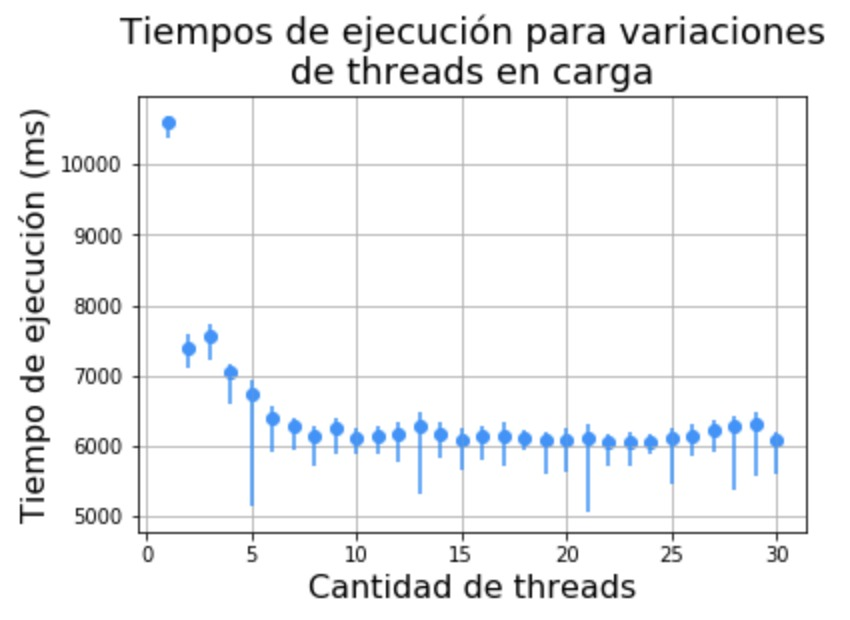
\includegraphics[scale=0.275]{graphs/threadsCarga.jpeg}
        \caption{Rendimiento según cantidad de threads en la carga de archivos (en $ms$)}
        \label{res-carga}
    \end{subfigure}
    \begin{subfigure}{.5\textwidth}
        \centering
        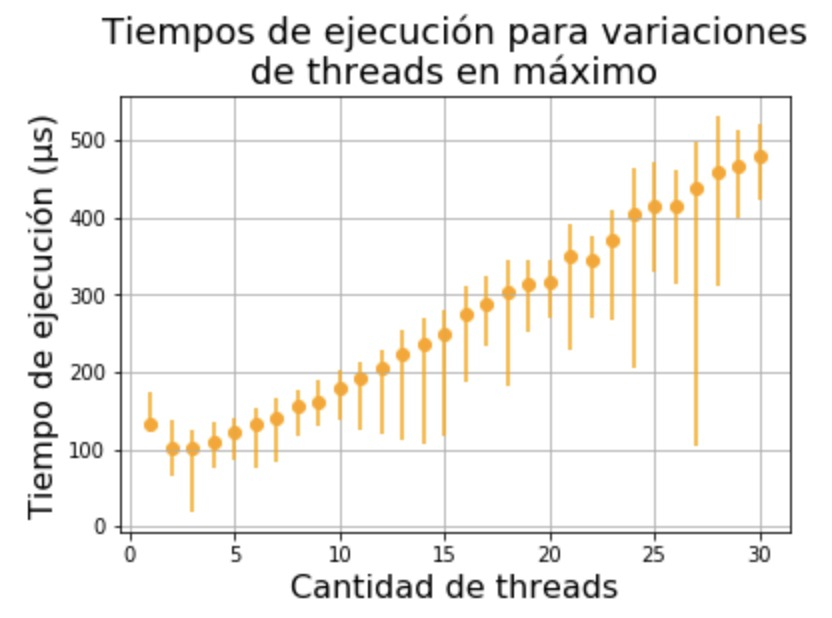
\includegraphics[scale=0.275]{graphs/threadsMaximo.jpeg}
        \caption{Rendimiento según cantidad de threads en la búsqueda del máximo (en $\mu s$)}
        \label{res-max}
    \end{subfigure}
\end{figure}

Por un lado, podemos observar que los resultados planteados para la búsqueda del máximo se condicen perfectamente con las hipótesis planteadas en \ref{hipotesis}.

Sin embargo, para el análisis de rendimiento empleado para la carga de archivos, notamos que la hipótesis planteada difiere ampliamente de los resultados obtenidos. Esto podría explicarse puesto que las operaciones predominantes en la carga de archivos resultan las de \textit{Entrada/Salida}. Por lo tanto, a diferencia de los utilizados para la búsqueda del máximo, estos threads se bloquearán esperando los resultados de sus peticiones a memoria, y esto hace posible que los threads dejen de ``sabotearse'' los unos a los otros, puesto que se bloquearían y así cederían su tiempo de procesamiento a otros threads que ya cuenten con los resultados de sus llamados a memoria.

De esta forma, podemos entender que el rendimiento de la carga de archivos mejore para cantidades de threads superiores a la cantidad de núcleos lógicos disponibles. Más aún, notamos que en los resultados no es posible apreciar una desmejora a partir de cierto punto, si no que luego de los $10$ threads la performance parecería ser más bien constante. Esto es nuevamente razonable, pues podemos suponer que el factor de mejora dadas las cuestiones de \textit{Entrada/Salida} producidas por el aumento de threads se encuentra en un orden equivalente al factor negativo generado por el ``sabotaje'' de los threads entre sí, produciendo una constante.

\subsubsection{Trabajos futuros}

De la investigación y los resultados propuestos se desprenden algunas dudas y cuestiones que sería interesante profundizar a futuro. Por ejemplo, analizar el comportamiento de los experimentos planteados bajo distintas condiciones de ejecución, en sistemas con mayor y menor cantidad de núcleos lógicos que los utilizados. 

Por otro lado, también sería interesante observar los resultados más allá de los $30$ threads, y además analizar la conducta del programa en la carga para distinta cantidad de archivos, y en la carga y la búsqueda del máximo para archivos de distintas características y tamaños.

Finalmente, para ayudar a entender los resultados de aumentar la concurrencia para la carga de archivos, podría ser útil realizar un \textit{profiling} más minucisoso, para así poder saber de forma más precisa cuánto tiempo pasaron los threads en \textit{I/O wait}.

\section{Conclusiones}

En base a la experimentación propuesta y los resultados obtenidos, se puede concluir que el multithreading resulta una notable y poderosa herramienta, a tener en cuenta a futuro con el fin de mejorar el rendimiento de programas. Resulta destacable la gran mejoría vista en los resultados, producto del incremento del grado de threads utilizados. Sin embargo, es importante utilizarla a discreción, pues no siempre aumentar la cantidad mejorará la performance y hasta podría pasar que esta empeore como se puede apreciar en el caso de la búsqueda de máximos, en la figura \ref{res-max}.

Además, notamos que las cuestiones de \textit{Entrada/Salida} suponen un factor importante a tener en cuenta al determinar la cantidad de threads a utilizar, junto con la cantidad de núcleos lógicos disponibles en el procesador sobre el que el programa correrá.

Finalmente, destacaremos que la concurrencia no deja de traer sus propios problemas, a pesar de sus grandes mejoras en rendimiento. Sin embargo, estos pueden ser evitados mediante el uso de las \textit{primitivas de sincronización} adecuadas para evitar las condiciones de carrera sin afectar demasiado la contención de recursos, con el fin de preservar el rendimiento del programa.

\end{document}
